\documentclass[letterpaper, 12pt]{article}
\usepackage[letterpaper, top=2.5cm, bottom=2.5cm, left=3cm, right=3cm]{geometry} %margenes
\usepackage[backend=biber]{biblatex}\addbibresource{bibliografia.bib} %manejo de bibliografía (BORRAR SI NO ES NECESARIO)
\usepackage[utf8]{inputenc} %manejo de caracteres especiales
\usepackage[spanish]{babel} %manejo de encabezados de inglés a español
\usepackage{fancyhdr} %formato de los encabezados de página
\usepackage{ragged2e} %alineado real justficado
\usepackage{graphicx} %manejo de imagenes
\usepackage{amsmath} %manejo de notación matemática
\usepackage{mathtools} %manejo de notación matemática
\usepackage{amssymb} %manejo de simbología
\usepackage{float} %centrado de imaene
\usepackage{hyperref} %manejo de enlaces e hipervínculos

\hypersetup{
  colorlinks   = true, %Colours links instead of ugly boxes
  urlcolor     = blue, %Colour for external hyperlinks
  linkcolor    = blue, %Colour of internal links
  citecolor   = red %Colour of citations
}

\pagestyle{fancy}
\fancyhf{}
\rfoot{\thepage}

\nocite{*}

\begin{document}
    
    %PORTADA
    \begin{titlepage}
        \begin{figure}[ht]
            \centering
            
\includegraphics[width=15cm]{logosITT.png}
        \end{figure}
        \centering
        {\scshape\LARGE Tecnológico Nacional de México\\Instituto Tecnológico de Tijuana\par}
        \vspace{1cm}
        {\scshape\Large Fundamentos de Bases de Datos\par}
        \vspace{1cm}
        {\scshape\Large Unidad 4\par}
        \vspace{1.5cm}
        {\huge\bfseries Investigación de Conceptos Básicos de la Unidad 4\par}
        \vspace{2cm}
        {\Large\itshape C. Abraham Jhared Flores Azcona\\19211640\par}
        \vfill
        Profesora: \par
        M.C. María Magdalena Serrano Ortega
    
        \vfill

        {\large 12 de mayo de 2021}
    \end{titlepage}

    %indices
    \newpage
        \thispagestyle{empty}
        \tableofcontents %indice de contenidos
        \listoffigures %indice de figuras

    %cuerpo
    \newpage
    \begin{justify}
        \setcounter{page}{1}
        \thispagestyle{fancy}
        \lhead{\textbf{Conceptos Básicos}}
        \section{Introducción}
        \justify
        En esta breve investigación, se explican los conceptos relacionados a la normalización de las bases de datos, los cuales son
        de suma importancia para comprender de mejor manera la unidad 4 de la materia.
        \section{Normalización de Bases de Datos}
        \justify
        A grandes rasgos, es una técnica de diseño de bases de datos que reduce la redundancia de datos y elimina características no deseadas
        como las anomalias de inserción, eliminación y actualización. Dichas reglas dividen tablas grandes en tablas pequeñas y las enlaza con
        usando relaciones. Su propósito es el de eliminar datos redundantes y que los mismos se almacenen lógicamente.
        \begin{figure}[H]
            \centering
            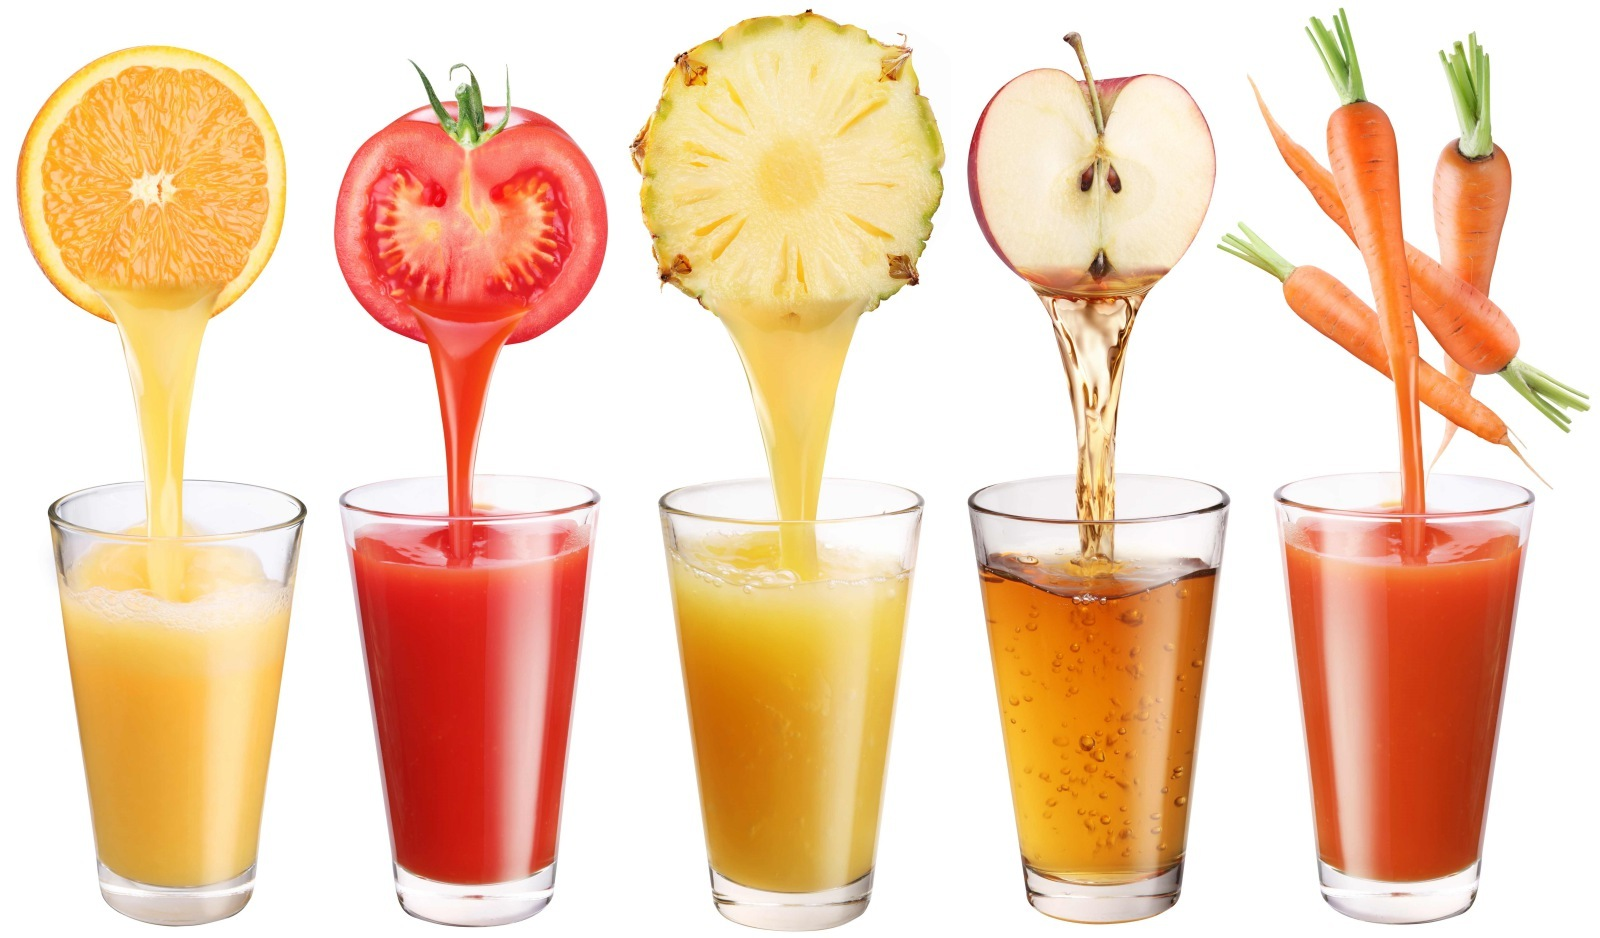
\includegraphics[width=10cm,height=6cm]{frutas.jpg}
            \caption{Se puede considerar la normalización como el exprimir el zumo de las frutas.}
        \end{figure}
        \justify
        De manera mas técnica, los datos redundantes desperdician espacio en disco y crean problemas de mantenimiento. Si es necesario cambiar los datos
        que se encuentran en más de un lugar, los datos deben cambiarse exactamente de la misma forma en todas las ubicaciones. El cambio de dirección
        de un cliente es mucho más fácil de implementar si los datos se almacenan solo en la tabla clientes y en ninguna otra parte de la base de datos.
        \section{Dependencias Funcionales Transitivas}
        \justify
        Brevemente, es cuando se cambia una columna no-clave, puede causar que otras columnas no-clave cambien sus valores
        \begin{figure}
            \centering
            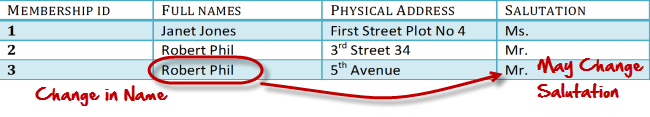
\includegraphics[width=12cm,height=6cm]{transitive_functional_dependencies.png}
            \caption{Ejemplo breve de las Dependencias Funcionales Transitivas}
        \end{figure}
        \justify
        Como se señala en la imágen en inglés, si se cambia el nombre, puede cambiar el saludo.
        \section{Primera Forma Normal}
        \justify
        Básicamente, se toma en cuenta lo siguiente:
        \begin{itemize}
            \item Cada celda de la tabla solo debe contener un solo valor.
            \item Cada registro necesita ser único.
            \item Se eliminan grupos repetidos en valores individuales.
            \item Se crea un tabla separada for cada conjunto de datos relacionados.
            \item Se identifica cada conjunto de datos relacionados con una llave primaria.
        \end{itemize}
        Dada la siguiente tabla:
        \begin{figure}[H]
            \centering
            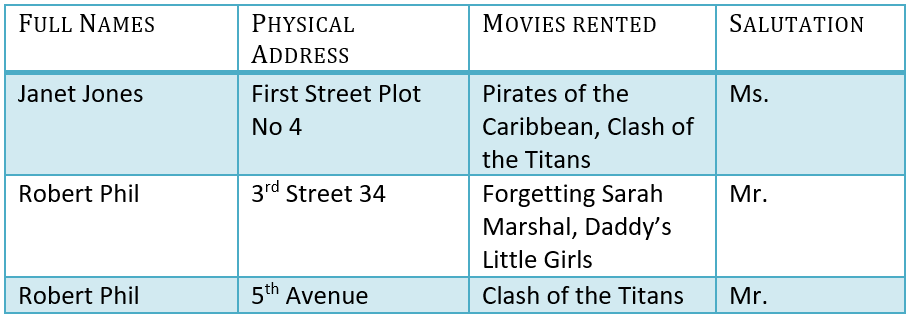
\includegraphics[width=10cm,height=6cm]{tabla-nonormalizada.png}
            \caption{Tabla no normalizada.}
        \end{figure}
        \justify
        Su Primera Forma Normal es la siguiente:
        \begin{figure}[H]
            \centering
            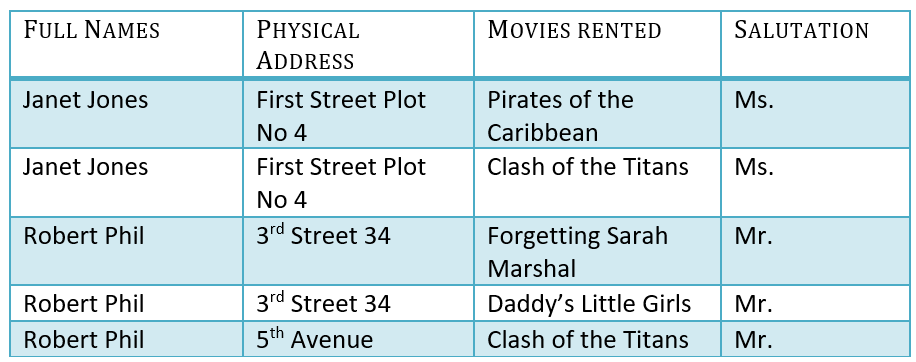
\includegraphics[width=10cm,height=6cm]{1NF.png}
            \caption{Tabla en 1ra. Forma Normal. Notese que solo es un dato en cada columna.}
        \end{figure}        

        \section{Segunda Forma Normal}
        \justify
        Se toma en cuenta lo siguiente:
        \begin{itemize}
            \item La tabla debe estar previamente en la 1ra. forma normal.
            \item Se define la columna de la llave primaria.
            \item Se crean tablas separadas para tipos de valores que aplican a múltiples registros.
            \item Se relacionan estas tablas con una llave primaria.
        \end{itemize}
        \justify
        Dada la siguiente tabla normalizada a la primera forma:
        \begin{figure}[H]
            \centering
            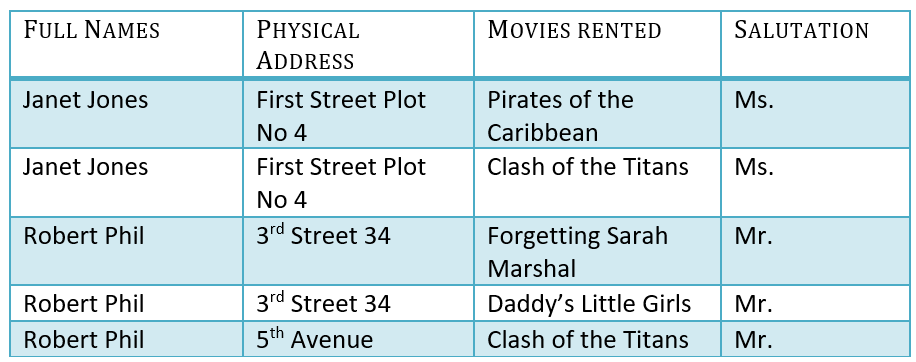
\includegraphics[width=10cm,height=6cm]{1NF.png}
            \caption{Tabla en 1ra. Forma Normal.}
        \end{figure}
        \justify
        Su Segunda Forma Normal es la siguiente:
        \begin{figure}[H]
            \centering
            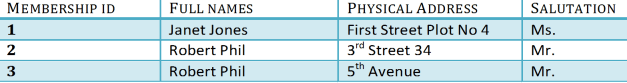
\includegraphics[width=12cm,height=4cm]{2NF.png}
            \caption{Tablas en 2da. Forma Normal.}
        \end{figure}
        \justify
        Notese que se dividó la tabla en 1ra. Forma Normal en dos tablas, donde la primera contiene la información de los miembros
        y la segunda tabla contiene información respecto a las películas rentadas. Se agrega una nueva colúmna llamada 
        \emph{Membership-id} el cual es la llave primaria de la primer tabla. En la segunda tabla, \emph{Membership-id} corresponde a la llave foranea.
        \section{Tercera Forma Normal}
        \justify
        Se tiene en cuenta lo siguiente:
        \begin{itemize}
            \item La tabla debe estar previamente en la 2da. forma normal.
            \item No debe tener Dependencias Transitivas Funcionales.
        \end{itemize}
        Dada la tabla normalizada a la segunda forma:
        \begin{figure}[H]
            \centering
            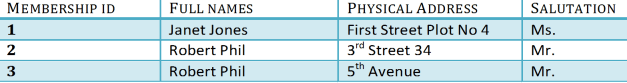
\includegraphics[width=14cm,height=4cm]{2NF.png}
            \caption{Tablas en 2da. Forma Normal.}
        \end{figure}
        \justify
        Su Tercera Forma Normal es la siguiente:
        \begin{figure}[H]
            \centering
            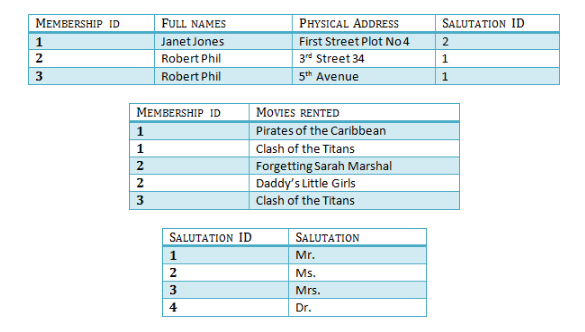
\includegraphics[width=10cm,height=8cm]{3NF.png}
            \caption{Tablas en 3ra. Forma Normal.}
        \end{figure}
        \justify
        Nótese que la tercer tabla se crea para almacenar los nombramientos y su llave primaria. El cambio de mayor notoriedad se encuentra en la
        primer tabla, donde los nombramientos se reemplazan por las llaves primarias anteriormente mencionadas.
        \section{Conclusión}
        \justify  
        El tener en cuenta dichas técnicas de normalización nos permiten tener una mejor curación de los datos que se manejan, y por ende, nos permiten
        un mejor flújo de trabajo con las bases de datos.
    \end{justify}

    %bibliografía
    \fancypagestyle{myplain} %estilo personalizado para la bibliografia
    {
      \fancyhf{}
      \renewcommand\headrulewidth{0pt}
      \renewcommand\footrulewidth{0pt}
      \fancyfoot[R]{\thepage}
    } %sin la barrita ni los encabezados, solo el numero de página en el pie derecho

    \newpage
        \thispagestyle{myplain} %ponerlo como \thispagestyle{myplain}
        \addcontentsline{toc}{section}{Referencias}
        \printbibliography
\end{document}